\documentclass{article}

\usepackage{a4wide}
\usepackage[utf8]{inputenc}
\usepackage[T1]{fontenc}
\usepackage[french]{babel}
\usepackage[babel=true]{csquotes} % guillemets français
\usepackage{graphicx}
\graphicspath{{Images/}}
\usepackage{color}
\usepackage{hyperref}
\hypersetup{colorlinks,linkcolor=,urlcolor=blue}

\usepackage{amsmath}
\usepackage{amssymb}


\title{Rapport Projet}
\author{Benjamin Singabrayen, L3 informatique}
\date{\today}

\begin{document}

\maketitle % pour écrire le titre


%% Le résumé:
\begin{abstract}
Dans ce rapport, je décris le code d'un programme choisi pour un projet et je donne également mes ressentis.
\end{abstract}

\section{Introduction}
\label{section:introduction} % pour faire référence à la section ailleurs (\ref{...} voir plus bas)

Ceci est le Latex que Mr.Etienne Payet nous a donné à rédiger qui conclut l'aboutissement de notre Projet.
Nous avons eu au départ le choix entre l'exercice 2.3 et 3.2 de notre TP Programmation Concurrente. J'ai choisis l'exercice 3.2
qui consite à écrire une programme,soit en java soit en python, qui affiche des balles en mouvements dans une fenêtre.J'ai bien sur
choisis de programmer en java car je suis plus à l'aise avec ce langage de programmation que python, c'est celui que je maitrise le plus.
Pourquoi ce choix? Tout simplement car l'exercice
sur les balles m'a parue dans un premier temps plus intéressant que l'exercice 2.3 qui consiste à créer deux threads producteurs et 
consommateurs qui se partagent une file. 
\vspace{5mm}\newline
Mon projet se compose de 5 fichiers java :
\begin{itemize}
\item Ball.java
\item Fenetre.java
\item GamePanel.java
\item Game.java
\item Tiimer.java
\end{itemize}

\begin{center}
  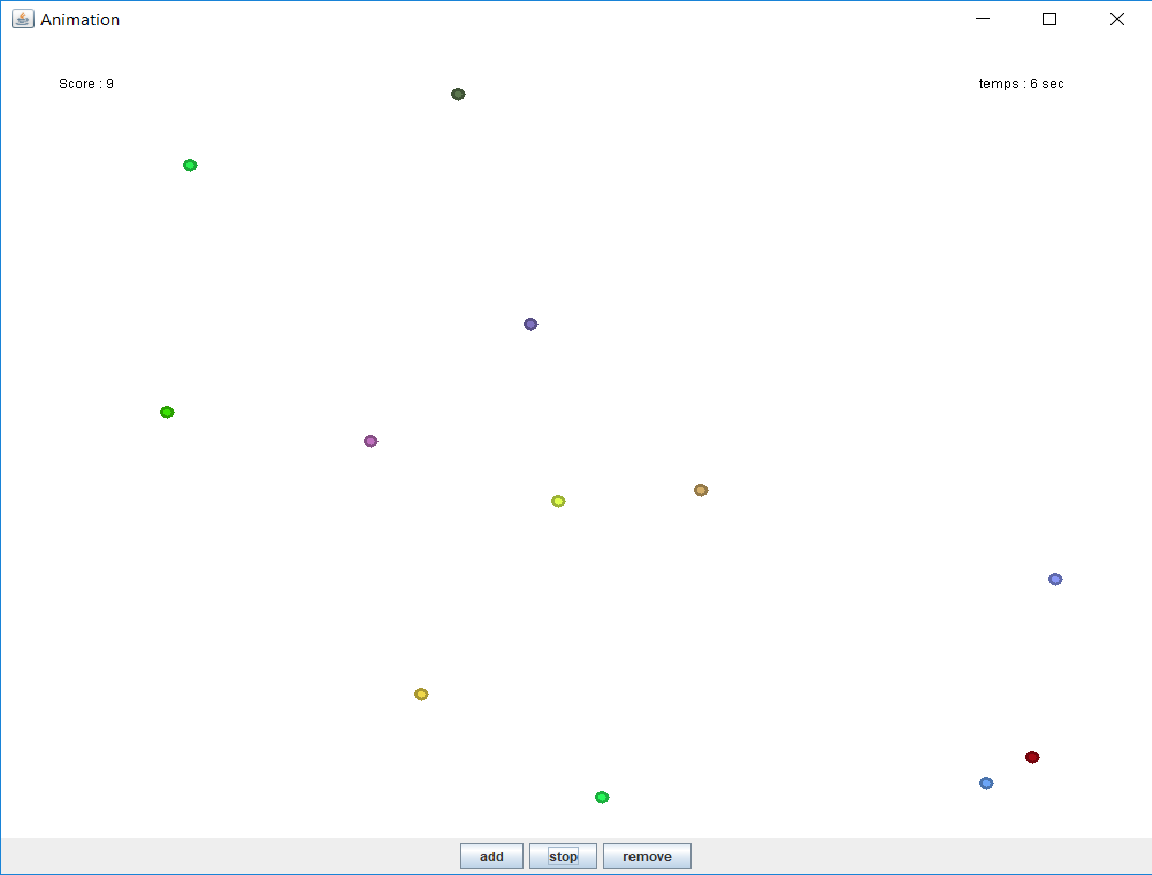
\includegraphics[scale=0.4]{Ballemouvement.png}
\end{center}

%%fin introduction

\section{Focus sur la partie codage}
\subsection{Class Ball}
% \ref{...} permet de faire référence à un élément défini
% ailleurs dans le document (voir \label{...} plus haut).
Je vais commencer par vous présenter ma classe Ball, car c'est aussi la première par laquelle j'ai commencé. \'A mon avis c'est celle qui contient le code le plus basique et c'est surtout l'objet de base de notre programme, sans elle notre affichage graphique serait tout banalement une simple fenêtre blanche. \vspace{5mm} \newline
Voici un aperçu de ma classe Ball:
\begin{center}
  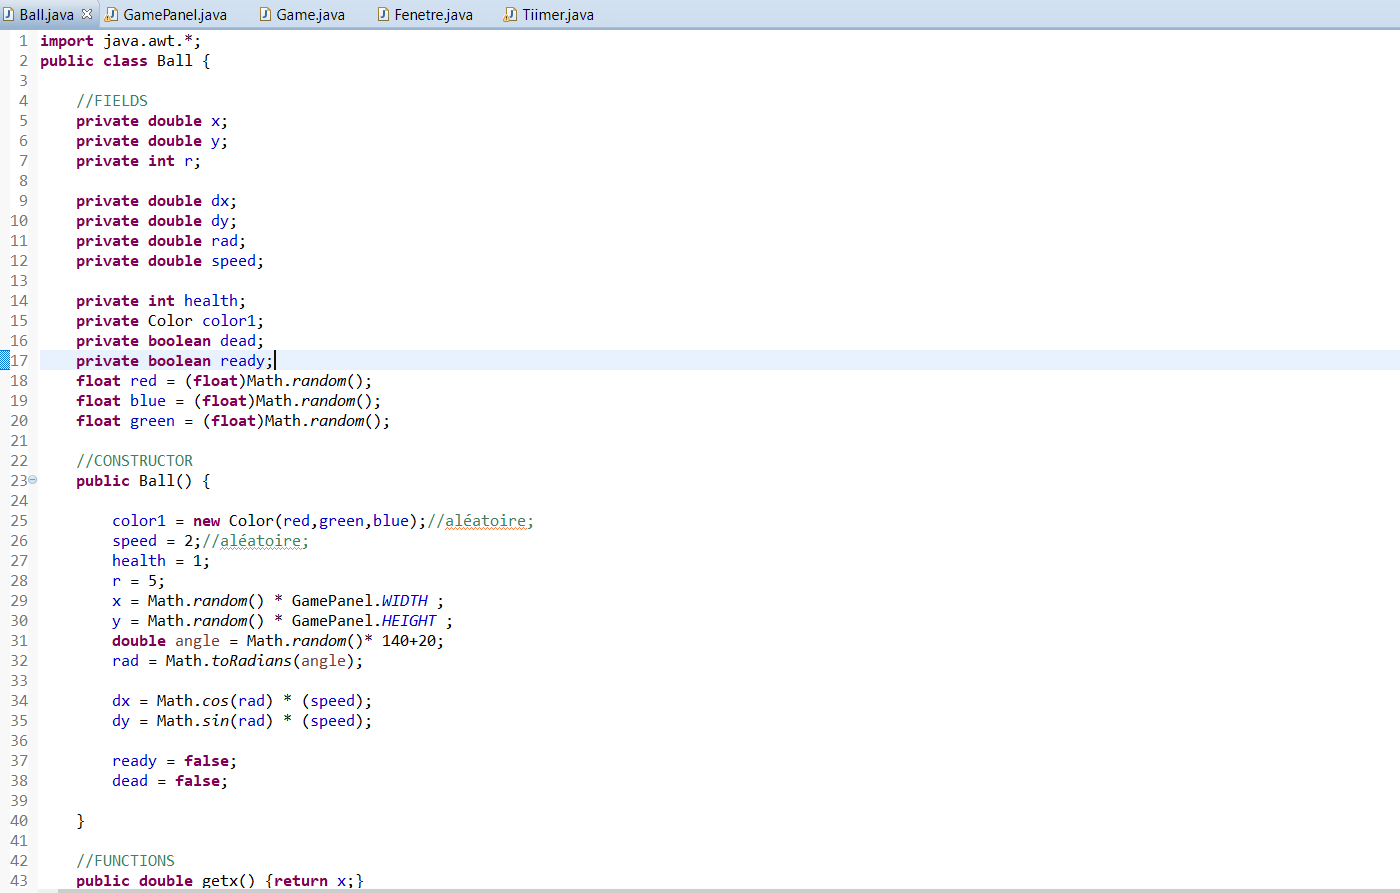
\includegraphics[scale=0.5]{BallApercu2.png}
\end{center}

%\newpage
Ma classe balle possède plusieurs paramètres:

\begin{enumerate}
\item Les paramètres de positions:
\begin{itemize}
\item double x: coordonnée x de l'objet Ball
\item double y: coordonnée y de l'objet Ball
\end{itemize}

\item les paramètres de déplacements:
\begin{itemize}
\item double dx: la coordonnée x d'une balle sera incrémentée de la valeur dx pour les déplacements horizontaux
\item double dy: la coordonnée x d'une balle sera incrémentée de la valeur dx pour les déplacements horizontaux
\item double speed : vitesse de déplacement de la balle
\end{itemize}

\item les paramètres qui gèrent la forme de la balle:
\begin{itemize}
\item int r : représente le rayon de l'objet Ball
\item Color color : couleur de notre objet Ball
\end{itemize}
\end{enumerate}

Les parties intéressantes et plut\^ot délicates à aborder selon moi dans cette classe Ball sont:
la fonction public void update() et et l'initialisation de la couleur de la balle avec une couleur aléatoire dans le constructeur de Ball.
\newpage

Le code pour la couleur de la balle:
\begin{verbatim}
float red = (float)Math.random();
float blue = (float)Math.random();
float green = (float)Math.random();
	
public Ball(){
    color1 = new Color(red,green,blue);
}
\end{verbatim}
Les trois variables red, blue, green initialisées par un nombre flottant aléatoire entre 0 et 1( (float)Math.random(); ) permet d'obtenir des teints de couleur rouge,vert et bleu différents pour chaque paramètre lors de la création de l'objet Color(red,green,blue) dans notre constructeur Ball.
\vspace{5mm}

Le code qui permet de dessiner une balle en tant qu'élément graphique ci-dessous est la fonction qui sera appelée dans le panneau pour dessiner chaque balle de ma liste de balles:

\begin{verbatim}
public void draw(Graphics2D g){
    g.setColor(color1);
    g.fillOval((int) (x-r), (int)(y-r), 2*r, 2*r);
    g.setStroke(new BasicStroke(3));
    g.setColor(color1.darker());
    g.drawOval((int) (x-r), (int)(y-r), 2*r , 2*r);
    g.setStroke(new BasicStroke(1));
}
\end{verbatim}

Enfin la dernière partie et la plus difficile de cette classe est celle qui gère les mouvements, est la fonction public void update()
son code est le suivant :

\begin{verbatim}
public void update() {
    x += dx;
    y += dy;	
	
    if(x < r && dx < 0) dx = -dx;
    if(y < r && dy < 0) dy = -dy;
    if(x > GamePanel.WIDTH -r && dx > 0) dx = -dx;
    if(y > GamePanel.HEIGHT -r && dy > 0) dy = -dy;
}
\end{verbatim}
Dans cette fonction on change les coordonnées pour faire bouger la balle, en additionnant  dx et dy respectivement à x et y. Ce changement de coordonnées permet de déplacer la balle dans le panneau;la balle bouge des coordonnées x en x+dx et des coordonnées y en y+dy. Ensuite dans la deuxième partie de ce code, on a crée des conditions pour prendre en compte les rebonds des balles sur les bords de notre panneau.
\begin{enumerate}
\item i\'ere condition if
\begin{itemize}
\item test de la condition : la balle se déplace à gauche et sa coordonnée x est inférieure à son rayon
\item conséquence: la balle se déplace à droite
\end{itemize}

\item i\'eme condition if
\begin{itemize}
\item test de la condition : la balle se déplace vers le haut et sa coordonnée y est inférieure à son rayon
\item conséquence: la balle se déplace vers le bas
\end{itemize}\newpage

\item i\'eme condition if
\begin{itemize}
\item test de la condition : la balle se déplace à droite et sa coordonnée x est supérieure à (la largeur du panneau - le rayon de la balle)
\item conséquence: la balle se déplace à gauche en x
\end{itemize}

\item i\'eme condition if
\begin{itemize}
\item test de la condition : la balle se déplace vers le bas et sa coordonnée y est supérieure à (la hauteur du panneau - le rayon de la balle)
\item conséquence: la balle se déplace vers le haut
\end{itemize}

\end{enumerate}

\subsection{Class Timer}
\vspace{5mm}
\begin{center}
  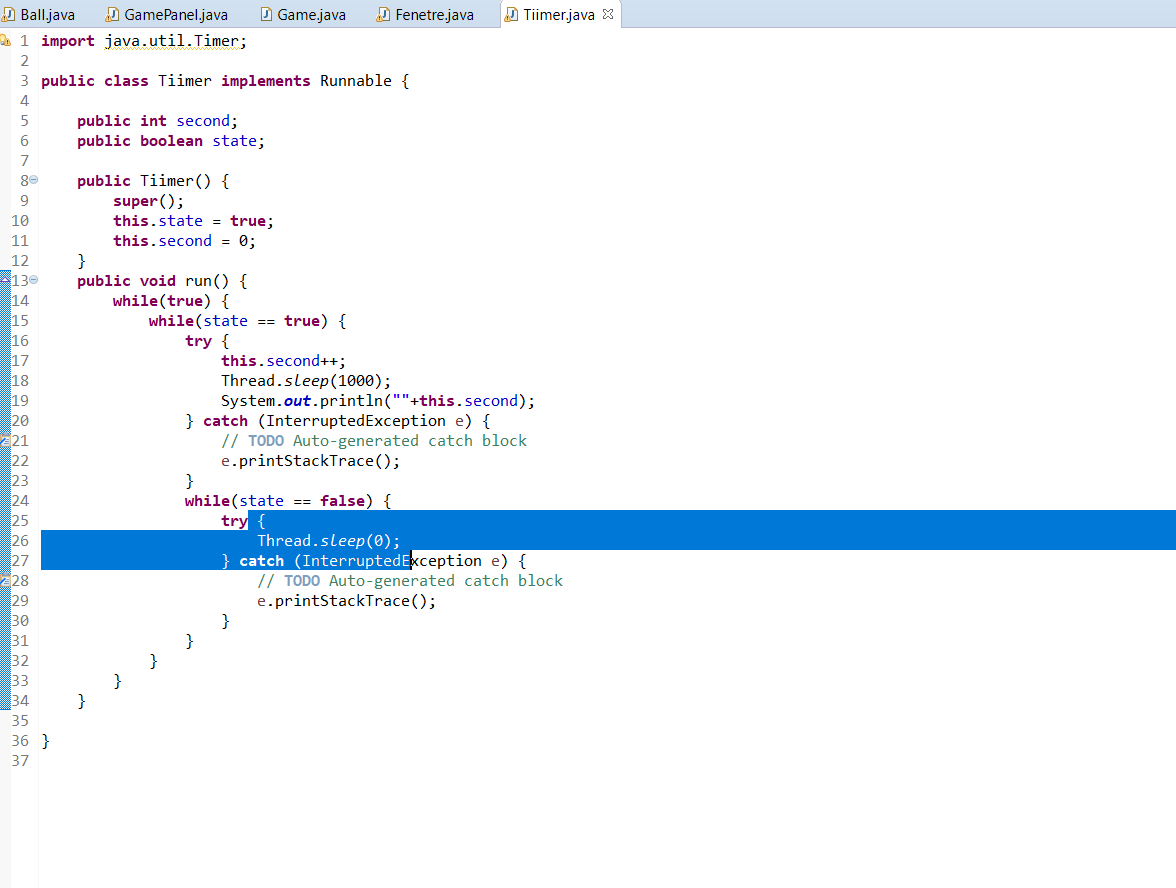
\includegraphics[scale=0.5]{Tiimer.png}
\end{center}
\vspace{1mm}
Mon objet timer possède deux paramètres:
\begin{itemize}
\item int second;
\item boolean state;
\end{itemize}
\vspace{5mm}

Ma classe Timer implémente l'interface Runnable. Elle possède une fonction run(). Sa fonction run() contient une boucle infini qui contient une boucle qui est exécutée si l'état du Tiimer est vrai, dans cette boucle les secondes s'incrémentent de 1 en 1 et mon Thread Tiimer dort pendant 1000 millisecondes. Si l'état du timer passe à faux une autre boucle dans la boucle while(state = true) est exécutée et le timer dort pendant 0 milliseconde. Faire cela permet de mettre le timer en pause quand l'état est à false. \newpage

\subsection{Class GamePanel}
\label{subsection:GamePanel}

Ma classe GamePanel est la plus importante, on dira que c'est le cerveau de mon code, C'est elle qui contient la majorité du code et qui gère l'affichage de mon Panel, l\'a o\'u mes balles se créent et se déplacent.\vspace{5mm} \newline
Aperçu de ma classe GamePanel:
\begin{center}
  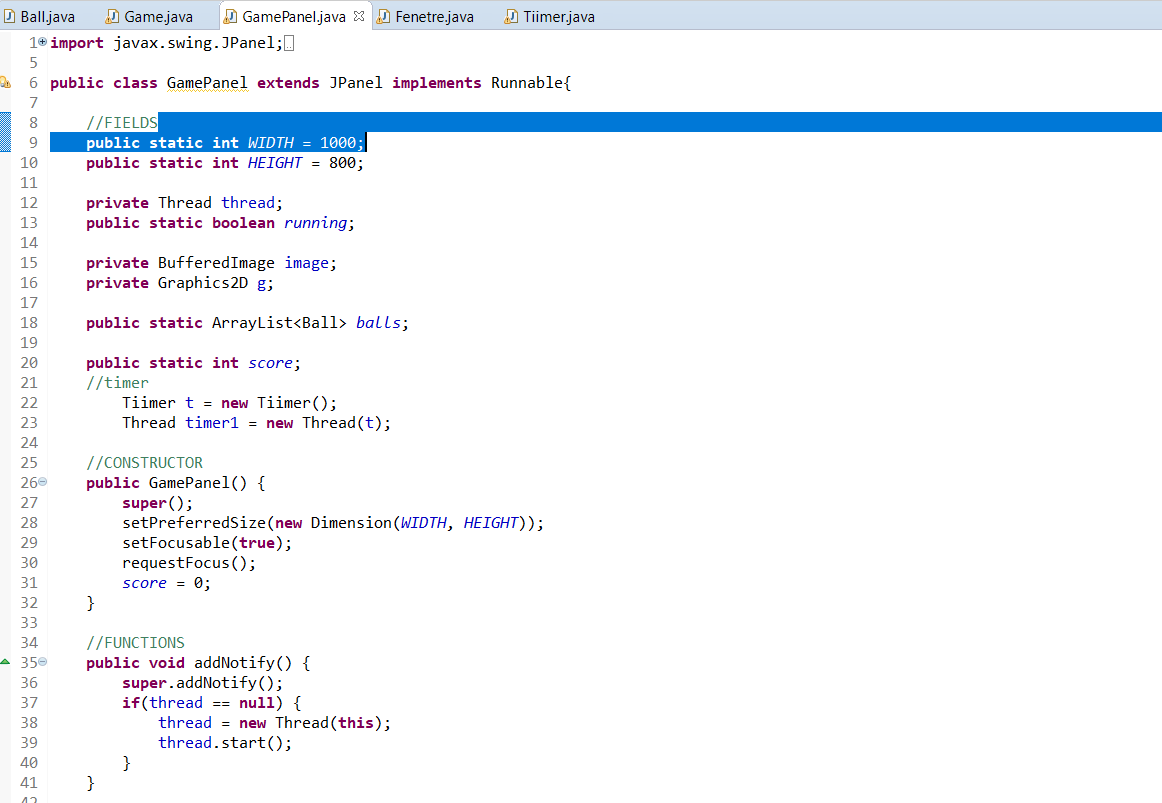
\includegraphics[scale=0.6]{GamePanelApercu.png}
\end{center}

On va commencer tout d'abord par la fonction run() du thread. Cette fonction est basée sur le même principe que celui du timer.

\begin{verbatim}
public void run() {
    running=true;
    //lancer chrono
    timer1.start();
    image = new BufferedImage(WIDTH, HEIGHT, BufferedImage.TYPE_INT_RGB);
    g = (Graphics2D) image.getGraphics();
    balls = new ArrayList<Ball>();
    // balls number instance
    for(int i = 0; i <30; i++) {
    balls.add(new Ball());
    }
    while(running) {
        gameUpdate();
        gameRender();
        gameDraw();
        //System.out.println(running);
        try {
            Thread.sleep(3);
        }catch(InterruptedException e) {
            e.printStackTrace();
        }
        //sleep my thread
            while(!running) {
                try {   // thread bug processeur boucle trop vite, pas vraiment de pause
                    System.out.println(running);
                    Thread.sleep(1000);
                   System.out.println(balls.size());
                    //add.addActionListener(new BoutonListener2());
                    //moins.addActionListener(new BoutonListener3());
                } catch (InterruptedException e) {
                    e.printStackTrace();
                }
            }
        }
    }
}
\end{verbatim}

Dans ce bout de code on passe l'état de running à true, on exécute le code de mon Thread timer , on crée un tableau qui va contenir l'ensemble de nos balles. Puis on exécute une boucle comme pour le thread Tiimer tant que running est vrai la boucle s'exécute et quand il est faux il exécute une autre boucle dans cette même boucle. \newline
Quand running est vrai il appelle la fonction locale gameUpdate(), gameRender() et gameDraw(), je n'entrerai pas en détail dans le fonctionnement de ces trois fonctions mais il faut savoir que gameRender() et gameDraw() gèrent l'affichage et la création de nos objets graphiques. Et la fonction gameUpdate() gère le mouvement des balles et la collision avec le mur grâce \`a l'appelle, pour chaque balle de notre tableau, de la fonction update() de notre classe Ball, elle gère aussi la collision entre chaque balle.\newline
Ensuite si running passe à false alors on entre dans la deuxième boucle qui elle ne met pas à jour les éléments graphiques. Quand cette boucle est exécutée les balles sont en pause, elles ne bougent plus, d'o\'u la présence du simple Thread.sleep() dans cette boucle.

\subsection{Class Fenetre}

Ma classe Fenêtre permet de disposer mon Panel GamePanel et mes boutons startstop, add et remove. Les boutons seront affichés au sud de ma fenêtre et le GamePanel sera placé au centre de ma fenêtre.
J'ai mis une taille fixe à ma fenêtre car je n'arrive pas à modifier la taille du GamePanel dynamiquement en agrandissant ou en réduisant la taille de la fenêtre.\vspace{5mm}

La classe pour mon écoute de bouton startstop:
\begin{verbatim}
class BoutonListener implements ActionListener{
    //Redéfinition de la méthode actionPerformed()
    public void actionPerformed(ActionEvent arg0) {
        if(GamePanel.running == true) {
            GamePanel.running = false;
            startstop.setText("stop");
            pan.t.state=false;
        } else {
            GamePanel.running = true;
            startstop.setText("start");
            pan.t.state=true;
        }
    }
}
\end{verbatim}

Lorsqu'on appuie sur le bouton auquel on ajoute cette écoute, dans notre Fenêtre c'est le bouton startstop, Si la variable running de notre GamePanel est à true, elle passe à false et les balles s'arrêtent de bouger et le timer arrête aussi le décompte du temps.\newline
Vice versa si il est à false il passe à true et les balles reprennent leur mouvement et le timer relance son décompte.\vspace{5mm}

La classe pour mon écoute de bouton add:
\begin{verbatim}
class BoutonListener2 implements ActionListener{ //ajouter un timer
//Redéfinition de la méthode actionPerformed()
    public void actionPerformed(ActionEvent arg0) {
        GamePanel.balls.add(new Ball());
        if (GamePanel.running == false){
            for(int i = 0; i < GamePanel.balls.size(); i++) {
                pan.gameRender();
                pan.gameDraw();
            }
        }
    }
}
\end{verbatim}

Lors de l'appui sur le bouton add, il y a un ajout de balle dans notre tableau de balle qui a été instancié dans mon GamePanel. Pour gérer l'affichage des balles lorsque mon thread GamePanel est en pause, j'ai rajouté les fonctions gameRender() et gameDraw() de ma classe GamePanel(vu dans la sous section~\ref{subsection:GamePanel}.\vspace{5mm}

La classe pour mon écoute de bouton remove:
\begin{verbatim}
class BoutonListener3 implements ActionListener{
    public void actionPerformed(ActionEvent arg0) {
        if (GamePanel.balls.size()!=0) {
            GamePanel.balls.remove(0);
            if (GamePanel.running == false){
                pan.gameRender();
                pan.gameDraw();
            }
        }
    }
}
\end{verbatim}

Le bouton remove fonctionne identiquement à celui de add, au lieu d'ajouter les balles on en enlève. Mais il reste une petite subtilité, si on enlève une balle alors que le tableau de balles est vide alors il y a une message d'erreur qui apparaît. J'ai réglé cette erreur en ajoutant une condition qui exécute la suppression d'une balle si et seulement si la longueur du tableau de balles est différente de zero. \newpage

\section{Conclusion}

Pour conclure il était intéressant de faire ce projet, il abordait toutes les notions qu'on a vu depuis la L2 sur java et également les Threads qu'on a étudiés en L3.\newline Le Thread étaient la principale difficulté rencontrée dans ce projet. Je n'étais pas très à l'aise au début avec cette notion, on ne l'a vu que très récemment. Mais ce fut une réelle expérience de pratiquer cela. Pour m'aider dans la programmation, j'ai utilisé la documentation java et le site OpenClassroom.\newline
Pour améliorer mon code, je pourrais rajouter une entrée clavier pour que l'utilisateur puisse spécifier combien de balle il veut créer au lancement du programme. J'avais pensé aussi à rajouter un bouton qui permet à l'utilisateur de changer la taille des balles, mais par respect de la consigne et du cahier des charges je ne l'ai pas fait.


\section{Bibliographie}
\nocite{*}
%%% La bibliographie:
\bibliographystyle{plain}
\bibliography{ma_biblio}


\end{document}
